\chapter{Background}
\label{background}
\section{Infandango}
Infandango is an automated web-based marking system for student submitted programming exercises. A student can view the list of warm-up, optional and core exercises and choose to submit a file for one of them. This file is then compiled and tested by Jester in a sandbox. Between the web frontend and Jester there is a PostgresSQL database which stores stores the source code of each submission and the score information for each marked submission.
Each question has a label: {\bf warmup} questions are simple questions which can be skipped if the user feels confident, {\bf core} questions are questions which the user is highly encouraged to try and may affect the end coursework mark, and {\bf optional} questions are provided for particularly interested students.
\subsection{Current feedback}
The primary source of feedback in Infandango is displayed in Figure \ref{fig:currentfeedback}. Each submission is marked with a set of JUnit tests and the fraction of these tests which are correct is displayed. This fraction is converted into a percentage and displayed on a red (0 - 40\%), orange (40\%-70\%) or green (70\%-100\%) background.
More general feedback is also available which displays similar information but the results are displayed by week rather than by question. 

\begin{figure}[p]
\centering
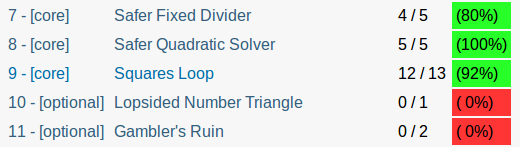
\includegraphics[width=0.8\textwidth]{currentfeedback.png}
\caption{This is a crop of what will be displayed to the user for a given week}
\label{fig:currentfeedback}
\end{figure}

\subsection{Current data}
The system has been used with the first year Java programming course at the University of Edinburgh, for a few years. The database information for these years has been kept and retains all the information about submissions: marks, submission time, number of resubmissions. This information for one year has been anonymised and made available for use. This has only happened for one year because the questions have changed since previous years and therefore the data would be inconsistent with the current questions.

\section{Literature}
Khan Academy\cite{khan_site} is a website which provides users with online education material:
\begin{quote}
Our online materials cover subjects ranging from math and finance to history and art.  With thousands of bite-sized videos, step-by-step problems and instant data\cite{ka_faq}
\end{quote}

%PUT IMAGE HERE FOR THE PARAGRAPH BELOW

A blog post\cite{khan_blog} written by David Hu about Khan Academy demonstrates that different feedback measures can affect user performance significantly. Khan Academy gives users certain kinds of exercises, for example choosing the approriate position on a number scale. It can then generate endless variations of this problem for the user to continue attempting until they are deemed proficient\footnote{
A proficiency is earned when a user is deemed to be "proficient" at a certain kind of exercise
}. The original Khan Academy system required a user to get 10 consecutive exercises of a certain type correct before they can be deemed proficient at that type of exercise. In an attempt to improve this system, a logistic regression model is used to calculate the probability that a user passes the next exercise successfully, with a threshold of 94\% representing the new proficieny level. Over a 6 day period 10\% of users tested the new method. Users of the new system earned 20.8\% more proficiences, attempted 15.7\% more exercises and required 26\% less exercises per proficiency. Hu summarises by saying the boost seems to come from allowing users to move on from exercises which they already proficient at, without requiring them to complete their streak thus wasting time on something they already understand.
Although the current system does not require perfection like Khan Academy did, it is possible that users are more reluctant to move on from exercises in which they get a minor error, and have just less than 100\%. Providing encouragement for the user to move on is one aim of this feedback design.
\subsection{Programming Assessment}
In {\it Automated Evaluation of Programming Assignments}\cite{automate_evaluation}, Kaushal and Singh describe various measures used as part of an automated marking system: regularity, efficiency, integrity and accuracy. Notably, Infandango only gives feedback on one of these areas, accuracy. The paper tracks the change in these measures as students use the system and find that there is a general improvement on all categories when feedback is based on these measurements. This shows that accuracy is not the only measurement that should be used to provide feedback and these are possibilities to be considered for Infandango.
\subsection{Machine Learning}
